%%%%%%%%%%%%%%%%%%%%%%%%%%%%%%%%%%%%%%%%%%%%%%%%%%%%%%%%%%%%%%%%%%%%%
%  Executar:   pdflatex
%              bibtex
%              pdflatex
%              pdflatex
%%%%%%%%%%%%%%%%%%%%%%%%%%%%%%%%%%%%%%%%%%%%%%%%%%%%%%%%%%%%%%%%%%%%%
%  DMTeX
%
%  Arquivo LaTeX para formatação de TCC, Mestrado e Doutorado
%  TCC, PPGM, PPGECE, ProfMat segundo as normas ABNT
%
%  Departamento de Matemática - UFSCar
%
%  Autor: Wladimir Seixas (seixas@ufscar.br)
%  Última atualização: 25/11/2021
%
%  Pacotes LaTeX que já estão carregados:
%
%     fontenc		helvet			inputenc		babel
%     microtype		geometry		setspace		graphicx
%     float			indentfirst		fancyhdr		etoolbox
%     caption		footmisc		enumitem		tocloft
%     amsmath		amsfonts		amssymb			amsthm
%     varioref		hyperref		color			backref
%     abntex2cite	appendix		mdframed        pdfpages
%     imakeidx
%
% Já estão pré-definidos os seguintes ambientes:
%
%	 \begin{teorema} .... \end{teorema}
%	 \begin{lema} .... \end{lema}
%	 \begin{proposicao} .... \end{proposicao}
%	 \begin{corolario} .... \end{corolario}
%	 \begin{definicao} .... \end{definicao}
%	 \begin{conjectura} .... \end{conjectura}
%	 \begin{exemplo} .... \end{exemplo}
%
%    Arquivos: dmtex.cls (template LaTeX)
%              monografia.tex 
%              referencias.bib (database BibTeX)
%              arquivosdmtex (diretório contendo logos)
%
%%%%%%%%%%%%%%%%%%%%%%%%%%%%%%%%%%%%%%%%%%%%%%%%%%%%%%%%%%%%%%%%%%%%%
%  PREENCHER OS APENAS OS CAMPOS DE INFORMAÇÕES
%  NÃO ALTERAR A ORDEM DOS COMANDOS. 
%  A CONFECÇÃO DO TRABALHO SEGUE A ORDEM DEFINIDA NA ABNT   
%%%%%%%%%%%%%%%%%%%%%%%%%%%%%%%%%%%%%%%%%%%%%%%%%%%%%%%%%%%%%%%%%%%%%

% CURSO          OPÇÃO
% TTC            tcc
% PROFMAT        profmat
% PPGECE         ppgece
% PGM-MESTRADO   mestre
% PGM-DOUTORADO  doutor

% Escolher uma das opções (% caso não se aplique).
%\documentclass[tcc,licenciatura]{dmtex}
\documentclass[tcc,bacharelado]{dmtex}
%\documentclass[ppgece]{dmtex}
%\documentclass[profmat,nofont]{dmtex}
%\documentclass[mestre,nofont]{dmtex}
%\documentclass[doutor,nofont]{dmtex}

% Coloque aqui outros pacotes LaTeX que você faça uso 
% (ver tabela acima)
\usepackage{enumitem}
% \usepackage[•]{•}

\newcommand{\sig}{$\sigma$-álgebra}
\newcommand{\sige}{\sigma(\mathcal{E}}
\newcommand{\muest}{\mu^*}
\newcommand{\muzero}{\mu_0}


\begin{document}

%%%%%%%%%%%%%%%%%%%%%%%%%%%%%%%%%%%%%%%%%%%%%%%%%%%%%%%%%%%%%%%%%%%%%
% DADOS: Preencher os campos comentando caso não se aplique.
%%%%%%%%%%%%%%%%%%%%%%%%%%%%%%%%%%%%%%%%%%%%%%%%%%%%%%%%%%%%%%%%%%%%%
 
% Título do trabalho
%\titulo{Título do trabalho $\mathbb{R}^n$}

% Autoria - seu nome
%\autoria{Nome do autor(a)}

% Ano da defesa depósito
%\ano{2021}

% Orientação - preencha o campo correspondente
%\orientador{Nome do Orientador}
%\orientadora{Nome da orientadora}
%\coorientador{Nome da coorientador}
%\coorientadora{Nome da coorientadora}

% A capa é um elemento OBRIGATÓRIO 
%\capa

%%%%%%%%%%%%%%%%%%%%%%%%%%%%%%%%%%%%%%%%%%%%%%%%%%%%%%%%%%%%%%%%%%%%%
% Elementos pré-textuais
% Parte que antecede o texto com informações que auxiliam na 
% identificação e utilização do trabalho.
%%%%%%%%%%%%%%%%%%%%%%%%%%%%%%%%%%%%%%%%%%%%%%%%%%%%%%%%%%%%%%%%%%%%%

% Folha de Rosto
% A folha de rosto é um elemento OBRIGATÓRIO que apresenta os 
% elementos essenciais para identificação do trabalho.
%\folhaderosto

% A ficha catalográfica, elemento OBRIGATÓRIO em trabalhos 
% acadêmicos, segundo a Norma ABNT - NBR 14724/2011 
% (Informação e documentação – Trabalhos acadêmicos – 
% apresentação), deve ser inserida no verso da folha de 
% rosto (na parte inferior). Para obter a ficha é necessário 
% que o autor preencha os campos com os dados da sua monografia, 
% o programa fará a formatação correta dos dados e irá gerar 
% a ficha catalográfica em um arquivo .PDF, fazendo o download 
% automático.
% Acesso: https://www.sibi.ufscar.br/servicos/gerador-de-ficha-catalografica
%\thispagestyle{empty}
%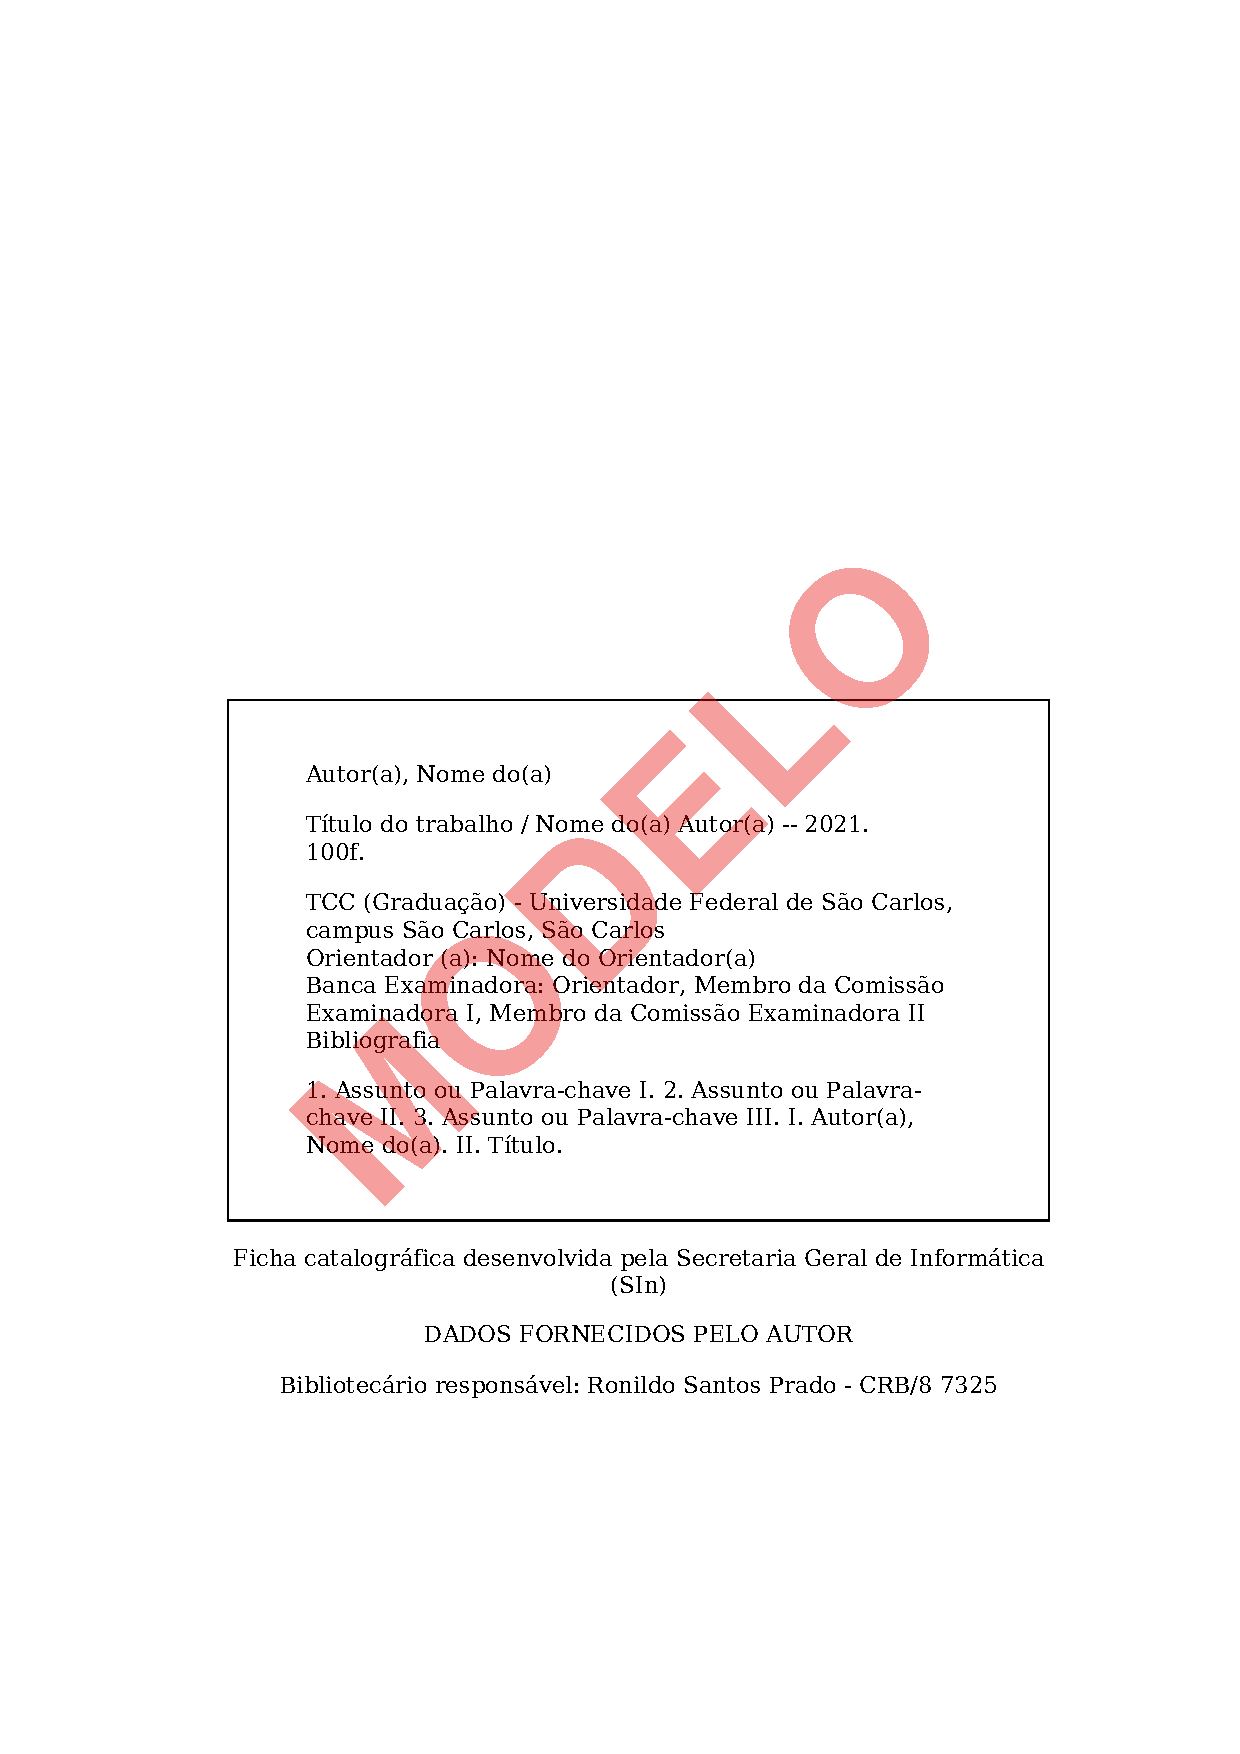
\includepdf[width=1.1\textwidth]{ficha-catalografica.pdf}

% A folha de aprovação é elaborada e fornecida pela 
% Coordenação de Curso (TCC) ou pelo 
% Programa de Pós-Graduação (PPGECE, Profmat ou PPGM)
%\thispagestyle{empty}
%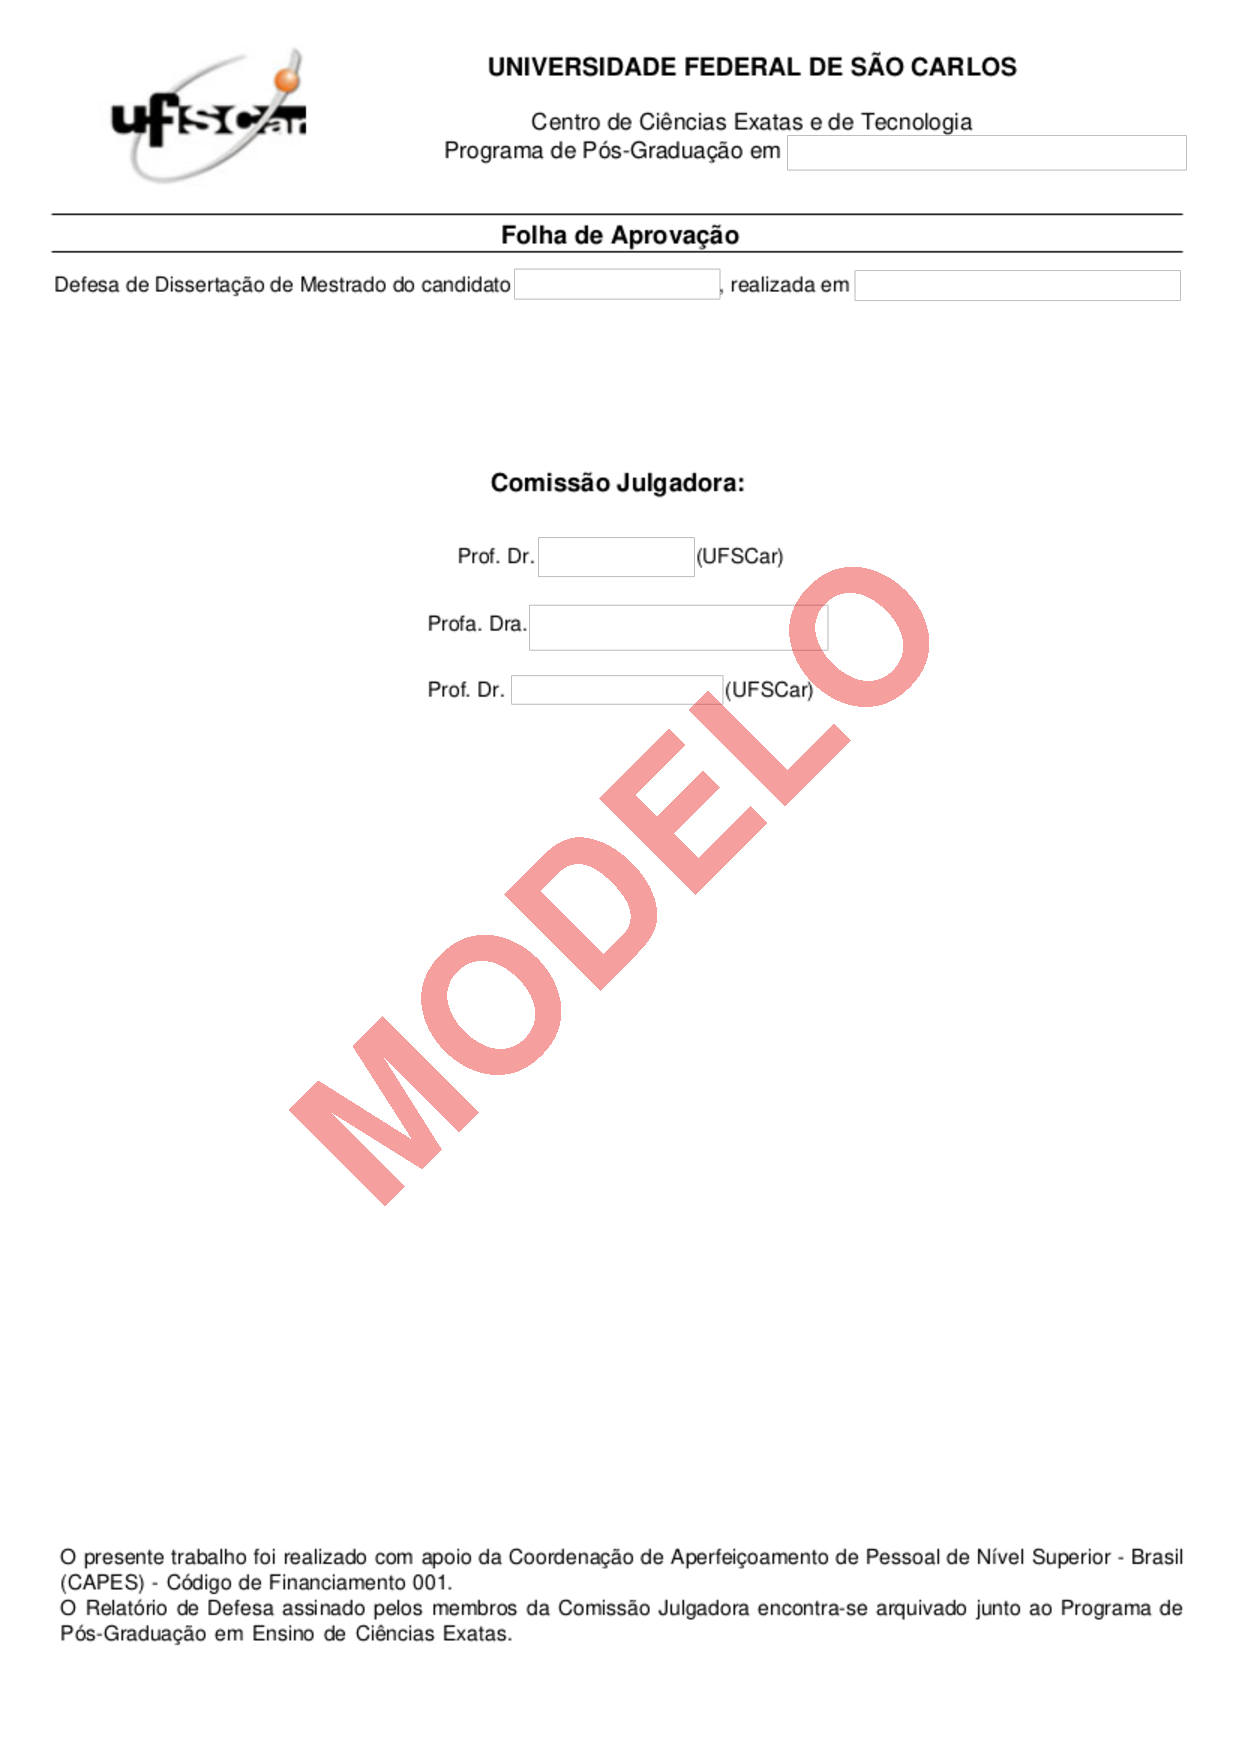
\includepdf[width=1.1\textwidth]{folhadeaprovacao.pdf}

% Dedicatória
% Comente o ambiente a seguir caso não fizer uso.

%\begin{dedicatoria}
%
%A dedicatória é um elemento OPCIONAL em que \\ o autor presta homenagem ou dedica seu trabalho.
%
%\end{dedicatoria}

% Agradecimento
% Comente o ambiente a seguir caso não fizer uso.

%\begin{agradecimentos}
%
%É um elemento OPCIONAL em que o autor faz agradecimentos aos que contribuíram de
%maneira relevante à elaboração do trabalho.
%
%\end{agradecimentos}

% Epígrafe
% É um elemento OPCIONAL em que o autor pode apresentar uma citação. 
% Deve-se fazer a indicação de autoria (citação) e a referência deve 
% constar na lista de Referências no final do trabalho.
% Comente o ambiente a seguir caso não fizer uso.
%\begin{epigrafe}
%Demonstração: Evidente \\
%\textbf{Elon Lages Lima} \cite[p. 154]{elon}.
%\end{epigrafe}

% Até 5 palavras-chaves - preencha os campos apropriados
% {1o campo-> em português}{2o campo-> em inglês}

%\palavrachaveI{Chave 1}{Key 1}
%\palavrachaveII{Chave 2}{Key 2}
%\palavrachaveIII{Chave 3}{Key 3}
%\palavrachaveIV{Chave 4}{Key 4}
%\palavrachaveV{Chave 5}{Key 5}

% Resumo na língua vernácula (Português)

%\begin{resumo}
%resumo
%\end{resumo}

% Resumo em língua estrangeira (Inglês)
% Versão do resumo em outro idioma para divulgação internacional. É permitido
% colocar o resumo em 1 (um) ou mais idiomas estrangeiros, caso julgue importante
% para divulgação do trabalho. Elaborar o Resumo em língua estrangeira de acordo
% com ABNT NBR 6028/2003. Abaixo do resumo devem ser colocadas as palavras-chave. 
% A indicação Keywords deve ser em negrito seguida de dois pontos e espaço. 
% Cada palavra deve ser separada uma da outra por ponto final.
% Para outra(s) língua(s) que não inglesa --> a ser implementado sob demanda 
% em razão do pouco uso.
% Entrar em contato com seixas@ufscar.br

%\begin{abstract}
%abstract
%\end{abstract}

% Lista de ilustrações
% Elemento OPCIONAL, precede o Sumário. São consideradas ilustrações: desenhos,
% esquemas, fluxogramas, fotografias, gráficos, mapas, organogramas, plantas,
% quadros, retratos e outras. Recomenda-se criar lista própria, sempre que o número
% de itens ultrapassar 5. Sua construção gráfica é a mesma do Sumário.

%\listoffigures   
%\cleardoublepage

% Lista de Tabelas
% Elemento OPCIONAL elaborada de acordo com a ordem apresentada no texto, tendo
% cada item designado por seu nome específico, acompanhado do respectivo número
% da folha ou página.

%\listoftables
%\cleardoublepage

% Sumário
% Elemento OBRIGATÓRIO que apresenta a enumeração das divisões, seções e outras
% partes do trabalho, na mesma ordem e grafia em que aparecem no texto.
% O Sumário deve ser elaborado de acordo com ABNT NBR 6027/2012.

%\tableofcontents
%\cleardoublepage

%%%%%%%%%%%%%%%%%%%%%%%%%%%%%%%%%%%%%%%%%%%%%%%%%%%%%%%%%%%%%%%%%%%%%
% Elementos textuais
% O texto é composto pela
%     Introdução, que apresenta os objetivos do trabalho, o
%     Desenvolvimento, que detalha a pesquisa ou estudo realizado e a​ 
%     Conclusão​ .
%%%%%%%%%%%%%%%%%%%%%%%%%%%%%%%%%%%%%%%%%%%%%%%%%%%%%%%%%%%%%%%%%%%%%

%\chapter{Intrudução} %%lembrar da introdução

\chapter{Espaços Mensuráveis}


\begin{definicao} \label{def1.1}
    
    Uma \textbf{álgebra} de subconjuntos de $X$ é uma família $\mathcal{B}$ de subconjuntos de $X$
    que é fechada para as operações elementares de conjuntos, ou seja: 
    
    \begin{enumerate}[label=(\roman*)]
        \item   Se $A \in \mathcal{B}$, então $A^c \in \mathcal{B}$
        \item Se $A, B \in \mathcal{B}$, então $A \cup B \in \mathcal{B}$
    \end{enumerate} 

    Note que como $ A \cap B = (A^c \cup B^c)^c $ e $A \setminus B = A \cap B^c$ para 
    quaisquer $A,B \in \mathcal{B}$, então tais operações de conjuntos também são fechadas 
    em $\mathcal{B}$, além disso como $\emptyset = X \cap X^c $ e $X = A \cup A^c$, nós também temos 
    que $\emptyset \in \mathcal{B}  $ e $ X \in \mathcal{B}$ .  
    Note também que, por associatividade, a união e intercecção de qualquer
    número finito de elementos de $\mathcal{B}$ está em $\mathcal{B}$.                                

\end{definicao}

\begin{definicao} \label{def1.2}
    
    Uma \textbf{$\sigma$-álgebra} é uma álgebra de subconjuntos de $X$ que também é fechada para a 
    união enumerável de subconjutos de $\mathcal{B}$, ou seja:

    \begin{enumerate}
        \item[(iii)] Se $ A_j \in \mathcal{B}, j = \{ 1,2,... \}$, então $ \bigcup\limits _{j=1} ^{\infty} A_j \in 
        \mathcal{B} $ 
    \end{enumerate}

    Note que como \( \bigcap _{j=1} ^{\infty} A_j = \big( \bigcup _{j=1} ^{\infty} A_j ^c \big) ^c  \), nós também temos que as $\sigma$-álgebras são fechadas 
    para as intersecções enumeráveis.

\end{definicao}

Abaixo seguem alguns exemplos de \sig .

\begin{exemplo} \label{ex1.1}
    
    Seja \(X=\{ a,b,c,d \} \),  $ \mathcal{B}_0 = \{ \emptyset, \{a,b\},\{c,d\}, \{a,b,c,d\} \}$
    é uma $\sigma$-álgebra, da mesma forma que $\mathcal{B}_1 = \{ \emptyset, X \} $ e 
    $\mathcal{B}_2 = 2^X $ também são $\sigma$-álgebras, ainda mais, $\mathcal{B}_1$ e 
    $\mathcal{B}_2$ são $\sigma$-álgebras para qualquer conjunto $X$, sendo $\{ \emptyset, X  \}$
    a menor e $2^X$ a maior $\sigma$-álgebra de qualquer conjunto $X$. 
\end{exemplo} 

\begin{exemplo} \label{ex1.2}
    Seja $X$ um conjunto não enumerável, então
    \[ 
    \mathcal{B} = \{ A \in X : A \ \text{é enumerável ou } A^c \ \text{é enumerável} \}
    \]
    é uma \sig. 
    
    \begin{proof}
        Tome $A \in \mathcal{B}$, $A$ é enumerável ou o $A^c$ é enumerável, se $A$ for enumerável, 
        nós teremos que o $(A^c)^c$ é enumerável logo $(A^c) \in \mathcal{B}$, se $A$ não for 
        enumerável, então $A^c$ é enumerável e logo $A^c$ também é elemento de $\mathcal{B}$, e a 
        primeira propriedade foi verificada.  \\
        Agora tome quaisquer $A_j \in \mathcal{B}$ tais que $A_j$ eles são contáveis, 
        então $ \bigcup _{i=1} ^{\infty}  A_j$ é enumerável já que a união enumerável de conjuntos 
        contáveis é enumerável. Tome agora $A_j \in \mathcal{B}$ tal que pelo ou menos um 
        $A_{j_0} ^c$ é enumerável , logo $(\bigcup_{i=1}^\infty A_j)^c 
        = \bigcap_{i=1}^\infty A_j ^c \subseteq A_{j_0}^c $, logo 
        $\bigcup_{i=1}^\infty A_j \in \mathcal{B}$ e provamos todas as propriedades 
    \end{proof}

\end{exemplo}

\begin{lema} \label{lema1.1}
    A intercecção de uma família de $\sigma$-álgebras é uma \sig 

    \begin{proof}
        Seja $ \{ \mathcal{B}_i : i \in \mathcal{I}  \} $ uma família não vazia de \sig s,
        de uma conjunto $X$ queremos mostrar 
        que $ \mathcal{B} = \bigcap_{i \in \mathcal{I}} \mathcal{B}_i $ é uma \sig. \\
        Tome $A \in \mathcal{B}$, então $ A \in \mathcal{B}_i , \forall i \in \mathcal{I}$ e
        $A^c \in \mathcal{B}_i, \forall i \in \mathcal{I}$, portanto $A^c \in \mathcal{B}$.
        Temos também que se $\forall j \in \mathbb{N}, A_ {j} \in \bigcap_{i \in \mathcal{I}} \mathcal{B}_i$ então 
        $\bigcup _{j = 1} ^{\infty} A_j \in \bigcap_{i \in \mathcal{I}} \mathcal{B}_i $ e demonstramos
        as duas propriedades de \sig, logo $\mathcal{B}$ é uma \sig . 
    \end{proof}

\end{lema}

\begin{definicao}
    
    Um \textbf{espaço mensurável} é uma dupla $(X,\mathcal{B})$, onde $X$ é um conjunto e $\mathcal{B}$
    uma $\sigma$-álgebra de subconjuntos de $X$. Os elementos de $\mathcal{B}$ são chamados 
    conjuntos mensuráveis. 

\end{definicao}

\begin{definicao}
    Uma \textbf{\sig \ gerada} por uma família $\mathcal{E}$ de subcontos de $X$ é a menor \sig \ de $X$ que contém $\mathcal{E}$ e será denotada por $\sigma (\mathcal{E})$. Por construção, podemos definir tal $\sigma$-álgebra da seguinte forma
    \[
    \sigma(\mathcal{E}) = \bigcap _{i \in \mathcal{I}} \{ \mathcal{B}_i : \mathcal{B}_i \ \text{é uma \sig \ e } \mathcal{E} \subseteq \mathcal{B}_i  \}    
    \]
\end{definicao}

    Note que $\sigma(\sigma(\mathcal{E})) = \sigma(\mathcal{E})$

\begin{definicao}
    Se $X$ é um espaço métrico, a \sig \ gerada pela família de  subconjuntos abertos de $X$ é chamada de \textbf{$\sigma$-álgebra de Borel}. A $\sigma$-álgebra de Borel na Reta e será denotada como $\mathcal{B}_{\mathbb{R}}$
\end{definicao} 



\begin{lema} \label{lema1.2}
    
    Se $\mathcal{E} \in \sigma(\mathcal{F}) $ então $ \sigma(\mathcal{E})  \subseteq  \sigma(\mathcal{F})$

    \begin{proof}
        
        $\mathcal{E}$ e $\mathcal{F}$ são famílias de subconjuntos de algum conjunto X. Note que se $\mathcal{E}$ está em $\sigma(\mathcal{F})$ então os elementos de $\mathcal{E}$ estão em $\mathcal{F}$ e $\mathcal{E} \subseteq \mathcal{F}$, o que implica que então $ \sigma(\mathcal{E})  \subseteq  \sigma(\mathcal{F})$

    \end{proof}

\end{lema}

\begin{proposicao} \label{prop1.1}
    
    A \sig \ de Borel em $\mathbb{R}$ pode ser gerada com
    
    \begin{enumerate}[label=(\roman*)]
        \item Os intervalos abertos $\mathcal{E}_1 = \{ (a,b) : a,b \in \mathbb{R} \}  $
        
        \item Os intervalos fechados $\mathcal{E}_2 = \{ [a,b] : a,b \in \mathbb{R} \}  $
        
        \item Os intervalos semi-abertos $\mathcal{E}_3 = \{ (a,b] : a,b \in \mathbb{R} \}  $ e $\mathcal{E}_4 = \{ [a,b) : a,b \in \mathbb{R} \}  $
        
        \item Os intervalos abertos ilimitados $\mathcal{E}_5 = \{ (a,\infty) : a \in \mathbb{R} \}$ e $\mathcal{E}_5 = \{ (\infty,a) : a \in \mathbb{R} \}$ 
        
        \item Os intervalos fechados e ilimitados $\mathcal{E}_6 = \{ (\infty,a] : a \in \mathbb{R} \} $ e $\mathcal{E}_7 = \{ [a, \infty) : a\in \mathbb{R} \}$
    \end{enumerate}

    \begin{proof}
        Seja $\tau$ a família dos conjuntos abertos de $\mathbb{R}$, por definição $\sigma(\tau)$ é a \sig \ de Borel. Provaremos cada item individualmente.
        
        \begin{enumerate}[label=(\roman*)]
        \item Como todos os elementos de $\mathcal{E}_1$ são abertos, então nós temos que $\mathcal{E}_1 \subseteq \tau$, logo $\sigma(\mathcal{E}_1) \subseteq \sigma(\tau)$. \\
        Para a inclusão inversa, basta lembrar que qualquer conjunto aberto de $\mathbb{R}$ pode ser escrito como a união enumerável de intervalos abertos de $\mathbb{R}$, portanto todos os elementos de $\tau$ estão contidos em $\sigma(\mathcal{E}_1)$ e pelo Lema \ref{lema1.2} nós temos que $\tau \in \sigma(\mathcal{E}_1)$ então $\sigma(\tau) \subseteq \sigma( \mathcal{E}_1) = \sigma(\mathcal{E}_1)$. \\
        Portanto $ \sigma(\tau) = \sigma( \mathcal{E}_1)$.
        
        \item Para todo $a,b \in \mathbb{R}, a < b$ nós temos que $(a,b)= \bigcup_{n=1} ^\infty [a + n^{-1}, b - n^{-1}] \in \sige _2) $, logo $\mathcal{E}_1 \in \sige _2)$ e portanto $\sige _1) \subseteq \sige _2)$. Também temos que $[a,b] = \bigcup _{n=1} ^\infty (a + n^{-1}, b - n^{-1}) $ e implicará que $ \sige _2) \subseteq \sige _1) $. Portanto $\sigma(\tau) = \sige _2 )$.
        
        \item Tomando $(a,b] = \bigcup _{n=1} ^\infty (a, b- n^{-1}) $ implicará que $\sige _3) \subseteq \sige _1) $ e tomando $(a,b) = \bigcap _{n=1} ^\infty (a,b - n^{-1} ]$ implica que $ \sige _1) \subseteq \sige _3)$. Portanto $ \sigma(\tau) = \sige _ 3)$. A demonstração para $\sige _ 4)$ é análoga.
        
        \item Tomando $(a, \infty) = \bigcup _{n=1} ^\infty (a, b + n) $ implica que $\sige _5) \subseteq \sige _1)$ e tomando $(a,b) = (a,\infty) - (b, \infty)$ implica que $\sige _ 1) \subseteq \sige _5)$. Portanto  $ \sigma(\tau) = \sige_5)$. A demonstração para $ \sige _ 6)$ é análoga.
        
        \item Tomando $[a, \infty ) = \bigcup _{n=1}^\infty [a, b + n]$ implica que $ \sige _ 6) \subseteq \sige _ 2)$ e tomando $ [a,b] = [a,\infty ) - [b,\infty)$
        implica que $\sige _ 2) \subseteq \sige _6)$. Portanto $\sigma(\tau) = \sige _ 6)$. A demonstração para $\sige _7) $ é análoga.
 
        \end{enumerate}

    \end{proof}

\end{proposicao}
       





\chapter{Espaços de medida}


\begin{definicao}
    
    Uma \textbf{medida} em um espaço mensurável $(X,\mathcal{B})$ é uma função $\mu: \longrightarrow [\mathcal{B}, +\infty]$ tal que:
    
    \begin{enumerate}[label=(\roman*)]
        \item $\mu(\emptyset) = 0 $;
        \item \textbf{($\sigma$-aditividade)}: $\mu( \bigcup _ {j=1} ^{\infty} A_j) = \sum ^{\infty} _{j=1} \mu (A_j) $ para quaisquer $A_j \in \mathcal{B} $ disjuntos dois a dois.   
    \end{enumerate}

Uma medida é \textbf{finitamente aditiva} se: 
\[ \mu( \bigcup _ {j=1} ^{n} A_j) = \sum ^{n} _{j=1} \mu (A_j) 
\]
onde $n \in \mathbb{N}$.


\end{definicao}
    
\begin{definicao}
    Um \textbf{espaço de medida} é uma tripla $(X,\mathcal{B},\mu)$, onde $\mu$ é uma medida no espaço mensurável $(X,\mathcal{B})$
\end{definicao}


\begin{teorema} \label{teo2.1}
    Seja $(X,\mathcal{B},\mu)$ um espaço de medida.

    \begin{enumerate}[label=(\roman*)]
        \item \textbf{(Monotonicidade)} Se $A,B \in \mathcal{B}$ e $A \subset B$, então $\mu(A) \leq \mu(B)$.

        \item \textbf{(Subaditividade)} Se $\{ A_n \}_1 ^{\infty} \in \mathcal{B}$, então $\mu(\bigcup _{k=1} ^{\infty} A_k) \leq \sum _{k=1} ^{\infty} \mu (A_k) $.
        
        \item \textbf{(Continuidade por baixo)} Se $\{ A_n \}_1 ^{\infty} \in \mathcal{B}$ e $A_1 \subset A_2 \subset ...$, então $\mu(\bigcup _{k=1} ^{\infty} A_k)= \lim _{k \longrightarrow \infty} \mu(A_k)  $.
        
        \item \textbf{(Continuidade por cima)} Se $\{ A_n \}_1 ^{\infty} \in \mathcal{B}$ e $E_1 \supset E_2 \supset ...$ e $\mu(A_1)< \infty$, então $\mu(\bigcap _{k=1} ^{\infty} A_k)= \lim _{k \longrightarrow \infty} \mu(A_k) $.
    \end{enumerate}

    \begin{proof}
        \begin{enumerate}[label=(\roman*)]
            \item $A \subset B$, então $B= B \setminus A \cup A$ onde $ B \setminus A \cap A = \emptyset$, portanto $\mu(B) =  \mu(B \setminus A) + \mu(A) \geq \mu(A)$ pois $\mu(B \setminus A) \geq 0$. 
            
            \item Seja $B_1=A_1$ e $B_k = A_k \ cup _{j=1} ^{k-1} A_j$ para $k>1$. Temos que $B_m \cap B_n = \emptyset$ se $m \neq n$ e $ \bigcup _{j=1} ^{n} A_j = \bigcup _{j=1} ^{n} B_j$  para todo $n$, ou seja, $ \bigcup _{j=1} ^{\infty} A_j = \bigcup _{j=1} ^{\infty} B_j$. Portanto, pelo item anterior, $ \mu(\bigcup _{j=1} ^{\infty} A_j) = \mu(\bigcup _{j=1} ^{\infty} B_j) \leq \sum _{j=1} ^{\infty} \mu(B_j) \leq \sum _{j=1} ^{\infty} \mu(A_j)$ .
            
            \item Seja $B_j = A_j \setminus A_{j-1}$, temos que $\bigcup _{j=1} ^\infty B_j = \bigcup _{j=1} ^\infty A_j $ e $B_m \cap B_n = \emptyset$ para todo $m \neq n$. Assim 
            \begin{align*}
                \mu(\bigcup _{j=1} ^\infty A_j) &= \mu(\bigcup _{j=1} ^\infty B_j) = \sum _{j=1} ^\infty \mu(B_j) 
                = \lim _{k \longrightarrow \infty} \sum _{j=1} ^k \mu(B_j) = 
                \lim _{k \longrightarrow \infty} \sum _{j=1} ^k \mu(A_j \setminus A_{j-1}) \\ 
                &= \lim _{k \longrightarrow \infty} \sum _{j=1} ^k \mu(A_j) - \mu(A_{j-1}) = \lim _{k \longrightarrow \infty} A_j.
            \end{align*}
            
            \item Seja $B_j = A_1 \setminus A_j$, já que $B_j \cap A_j = \emptyset$, então $\mu(A_1)=\mu(B_j \cup A_j)= \mu(B_j) + \mu(A_j)$ e $\bigcup  _{j=1} ^\infty B_j = A_1 \setminus \bigcap _{j=1} ^\infty A_j $, ou seja $\bigcap _{j=1} ^\infty A_j = A_1 \setminus  \bigcup  _{j=1} ^\infty B_j$, e como $B_1 \subset B_2 \subset ...$, pelo item anterior nós temos que $\mu(\bigcup  _{j=1} ^\infty B_j)= \lim _{n \longrightarrow \infty} \mu(B_n) = \lim _{n \longrightarrow \infty} \mu (A_1) - \mu(A_n)$. Portanto, como $\mu(A_1) < \infty$, nós obtemos que
            \[
                \mu(\bigcap _{j=1} ^\infty A_j) = \mu(A_1) - \mu(\bigcup  _{j=1} ^\infty B_j) = \mu(A_1) + \lim _{n \longrightarrow \infty} \mu (A_1) - \mu(A_n) =   \lim _{n \longrightarrow \infty} \mu(A_n).
            \]
            
            
             
        \end{enumerate}
    \end{proof}

\end{teorema}

\begin{definicao}
    Uma medida é completa se o seu domínio contém todos os subconjuntos do conjunto nulo, ou seja, $(X,\mathcal{B},\mu)$ um espaço de medida, $\mu$ é completa se, e somente se, $A \subseteq N \in \mathcal{B}$ e $\mu(N)=0$, então $A \in \mathcal{B}$. 
\end{definicao}

\begin{teorema}
    Seja $(X,\mathcal{B},\mu)$ um espaço de medida, $\mathcal{N}=\{ N \in \mathcal{B} : \mu(N)=0 \}$ e $ \overline{\mathcal{M}} = \{ A \cup B : A \in \mathcal{M} \ \text{e} \ B \in \mathcal{N} \}$. Então $\overline{\mathcal{M}}$ é uma \sig \ e existe uma única extensão $\overline{\mu}$ de $\mu$ para uma medida completa de $\overline{\mathcal{M} }$ 
\end{teorema}

\begin{definicao}
    Uma \textbf{medida exterior} em um conjunto não vazio $X$ é uma função $\mu^*: 2^X \longrightarrow [0,\infty]$ tal que 
\end{definicao}

\begin{enumerate}[label=(\roman*)]
    \item $\mu^*(\emptyset)=0$;
    \item \textbf{(Monótona)}  $A \subseteq B$, então $\mu^* (A) \leq \mu^*(B)$;
    \item \textbf{(Subaditividade enumerável)} $\mu^* (\bigcup _{j=1} ^\infty A_j) \leq \sum _{j=1} ^\infty \mu^* (A_j) $
\end{enumerate}

\begin{proposicao} \label{prop2.1}
    Seja $\mathcal{E} \subseteq 2^X$ uma família elementar e seja $\rho: \mathcal{E} \longrightarrow [0,\infty]$ tal que $\emptyset \in \mathcal{E}, X \in \mathcal{E} \ e \ \rho(\emptyset)=0$. Para todo $A \in X$, seja 
    \[
    \mu^*(A)= \inf \bigg\{  \sum _{j=1} ^\infty \rho(E_j): E_j \in \mathcal{E} \ \text{e} \ A \subseteq \bigcup_{j=1} ^\infty E_j \bigg\}  
    \]
    Então $\mu^*$ é uma medida exterior.
    
    \begin{proof}
        $\muest(\emptyset)=0$ pois basta tomar $E_j=\emptyset$ para todo $j$. Agora se $A \subseteq B$, então 
        \[
            A'=\bigg\{  \sum _{j=1} ^\infty \rho(E_j): E_j \in \mathcal{E} \ \text{e} \ A \subseteq \bigcup_{j=1} ^\infty E_j \bigg\} \supseteq \bigg\{  \sum _{j=1} ^\infty \rho(E_j): E_j \in \mathcal{E} \ \text{e} \ A \subseteq B \subseteq \bigcup_{j=1} ^\infty E_j \bigg\} = B'
        \]
        Como $A' \supseteq B'$ então $\inf A' \leq \inf B'$, ou seja, $\muest(A) \leq \muest(B)$
        Agora suponha que $\{ A_j \}_{j=1}^\infty \subseteq 2^X$ e fixe $\epsilon>0$. Pela definição de $\muest$, para cada um dos $j$ existe $\{ E_j ^k \}_{k=1} ^\infty \subseteq \mathcal{E}$ tal que $A_j \subseteq \bigcup _{k=1}^\infty E_j ^k$ e, pela definição de infimo, temos que $\sum _{k=1}^\infty \rho (E_j ^k) \leq \muest(A_j) + \epsilon 2^{-j }$. Tomando $A=\bigcup _{j=1}^\infty A_j$ nós temos que $A \subseteq \bigcup _{j=1}^\infty \bigcup _{k=1}^\infty E_j ^k$ e $\sum _{j=1}^\infty \sum _{k=1}^\infty \rho (E_j ^k) \leq \sum _{j=1}^\infty \muest(A_j) + \sum _{j=1}^\infty \epsilon 2^{-j }$ mas então $\muest(A) \leq \sum _{j=1}^\infty \muest(A_j) + \epsilon$ e como a escolha de $\epsilon$ foi arbitrária, nós concluímos a demonstração.
    \end{proof}

\end{proposicao}

\begin{definicao}
    Seja $\mu^*$ uma medida exterior em $X$, um conjunto $A \subseteq X$ é chamado de $\mu^*$ mensurável se, para todo $E \subseteq X$ 
    \[
        \mu^*(E)=\mu^*(E \cap A) + \mu^*(E \cap A^c). 
    \]
\end{definicao}

\begin{teorema}
    Se $\mu^*$ é uma medida exterior em $X$, a família $\mathcal{M}$ de conjuntos $\mu^*$ mensuráveis é uma \sig \ e a restrição de $\mu^*$ à $\mathcal{M}$ é uma medida completa.
\end{teorema}

\begin{definicao}
    Uma \textbf{pré-medida} em uma álgebra $\mathcal{A} \subseteq 2^X$ é uma função $\mu_0: \mathcal{A} \longrightarrow [0,\infty]$ tal que 
    \begin{enumerate}[label=(\roman*)]
        \item $\mu_0(\emptyset)=0$;
        \item \textbf{($\sigma$-aditividade)} $\{A_j\}_{j=1}^\infty$ uma sequência de conjuntos disjuntos dois a dois de $\mathcal{A}$ tais que $\bigcup _{j=1}^\infty A_j \in \mathcal{A}$, então $\mu_0  ( \bigcup _{j=1}^\infty A_j ) = \sum _{j=1}^\infty \mu_0(A_j)$.
    \end{enumerate}
\end{definicao}

\begin{proposicao}
    Seja $\mu_0$ uma pré-medida em $\mathcal{A}$ e $\mu^*$ definida assim como na proposição \ref{prop2.1} mas sobre $\mu_0$ ao invés de $\rho$ e sobre $\mathcal{A}$ ao invés de $\mathcal{E}$. Teremos então que 
    \begin{enumerate}[label=(\roman*)]
        \item $\mu^*$ restrita em $\mathcal{A}$ é igual a $\mu_0$;
        \item Todo conjunto em $\mathcal{A}$ é $\mu^*$ mensurável.
    \end{enumerate}
    \begin{proof}
        \begin{enumerate}[label=(\roman*)]
            \item Seja $E \in \mathcal{A}$ qualquer, temos que existe uma sequência de conjunto $\{A_j\}_{1}^\infty$ em $\mathcal{A}$ tal que $E \subseteq \bigcup _{j=1}^\infty A_j$. Seja $B_n = E \cap (A_n \setminus \bigcup _{j=1}^{n-1} A_j) $, então $B_r \cap B_s = \emptyset$ se $r \neq s$ e $E= \bigcup _{j=1}^\infty B_j$. Assim, $\muzero(E) = \sum _{j=1}^\infty \muzero(B_j) \leq \sum _{j=1}^\infty \muzero(A_j)$ pois $ \bigcup _{j=1}^\infty B_j \subseteq \bigcup _{j=1}^\infty A_j$ e pré-medidas são monótonas (a demonstração de tal fato é análoga a demonstração do item (i) do teorema \ref{teo2.1} . Portanto $\muzero(E)\leq \muest(E)$. Para a igualdade inversa, note que $E \subseteq E \cup \emptyset \cup \emptyset \cup ...$, e pela definição de $\muest$ nós finalmente obtemos que $\muest(E) \leq \muzero(E)$.
            
            \item Seja $A \in \mathcal{A}$ qualquer e $E \subseteq X$, fixe $\epsilon>0$, temos que existe uma sequência de conjunto $\{A_j\}_{1}^\infty$ em $\mathcal{A}$ tal que $E \subseteq \bigcup _{j=1}^\infty A_j$ e, pela definição de infimo, $\sum _{j=1}^\infty \muzero(A_j) \leq \muest(E) + \epsilon$. Como $\muzero$ é aditiva em $\mathcal{A}$ e como $(A_j \cap A) \cap (A_j \cap A^c) = \emptyset$ com $(A_j \cap A) \subseteq A \ \text{e} \ (A_j \cap A^c) \subseteq A$, então
            \begin{align*}
                \muest(E)+\epsilon \geq  \sum _{j=1}^\infty \muzero(A_j) &\geq \sum _{j=1}^\infty \muzero((A_j \cap A) \cup (A_j \cap A^c)) \\ &\geq \sum _{j=1}^\infty \muzero(B_j \cap A) + \sum _{j=1}^\infty \muzero(A_j \cap A^c) \\ &\geq \muest(A_j \cap A) + \muest (A_j \cap A^c)
            \end{align*}
            Como a escolha de $\epsilon$ foi arbitrária, nós obtemos um lado da igualdade.
            Quando ao outro lado da desigualde, como $E \subseteq (A_j \cap A) \cup (A_j \cap A^c)$ e como $\muest$ é aditiva, então $\muest(E) \leq \muest(A_j \cap A) + \muest (A_j \cap A^c)$

        \end{enumerate}
    \end{proof}
\end{proposicao}

\begin{definicao}
    Seja $(X, \mathcal{B},\mu)$ um espaço de medida. $\mu$ é dita \textbf{finita} se $\mu(X)<\infty$. $\mu$ é dita \textbf{$\sigma$-finita} se $\exists A_1, A_2, ... \in \mathcal{B}$ tal que $X=\bigcup _{j=1} ^\infty A_j$, onde $\mu(A_j)<\infty, \forall j = 1,2,...$ 
\end{definicao}

\begin{teorema} \label{teo2.4}
    Seja $\mathcal{A} \subseteq 2^X$ uma álgebra, $\muzero$  uma pré-medida em $\mathcal{A}$ e $\mathcal{M}$ \sig \ gerada por $\mathcal{A}$. Então existe uma medida $\mu$ em $\mathcal{M}$ cuja restrição em $\mathcal{A}$ é igual a $\muzero$. Além disso, qualquer outra medida $\nu$ em $\mathcal{M}$ que extende $\muzero$  será tal que $\nu(E) \leq \mu(E)$ para todo $E \in \mathcal{M}$, sendo igual caso $\mu(E)<\infty$. Se $\muzero$  for $\sigma$-finita, então existe uma única extensão de $\muzero$  para uma medida de $\mathcal{M}$
\end{teorema}



\chapter{Medida de Borel}

\begin{definicao}
    Uma \textbf{medida de Borel} é uma medida cujo domínio é uma \sig \ de Borel.
\end{definicao}


\begin{definicao}
    Seja $\mu$ uma medida de Borel em $\mathbb{R}$, a \textit{função de distribuição de $\mu$} é definida como 
    \begin{align*}
        F_{\mu}: \mathbb{R} & \longrightarrow \overline{\mathbb{R}} \\
                        x   & \mapsto \mu((-\infty,x]).
    \end{align*}
\end{definicao}

\begin{proposicao}
    Seja $F$ uma medida de distribuição de $\mu$, então $F$ é crescente e contínua à direita.
    \begin{proof}
        Seja $x,y \in \mathbb{R}$ tal que $x<y$, assim $(-\infty,x] \subset (-\infty,y]$ e pelo item (i) teorema \ref{teo2.1} do último capítulo, $\mu((-\infty,x])\leq \mu((-\infty,y])$. Portanto $F(x)=\mu((-\infty,x]) \leq \mu((-\infty,y])=F(y)$ e $F$ é crescente. \\
        Seja $\{x_n\}_1 ^\infty \subset \mathbb{R}$ uma sequência convergente a $x$ pela direita, ou seja, $ x_{j+1} \leq x_j $ para todo $j$. Mas então  $(-\infty,x_{j+1}] \subseteq (-\infty,x_{j}]$ para todo $j$ e, pelo item (iv) do teorema \ref{teo2.1} do capítulo anterior, $ \lim _{n \longrightarrow \infty} \mu((-\infty,x_n]) = \mu(\bigcap _{j=1} ^\infty (-\infty,x_j]) = \mu((-\infty,x])=F(x)$. Como a escolha de $\{x_n\}_1 ^\infty$ foi arbitrária, então $F(x)$ é contínua. 
    \end{proof}
\end{proposicao}

\begin{proposicao} \label{prop3.2}
    Seja $\mathcal{E} = \{(a,b],(a,\infty),\emptyset: -\infty \leq a < b < \infty \ ; \ a,b \in \overline{\mathbb{R}}\}$ o conjunto dos intervalos semi-abertos à esquerda de $\mathbb{R}$. Então o conjunto $\mathcal{A}$ da união contável de elementos de $\mathcal{E}$, ou seja, $\mathcal{A}=\{ \bigcup _{i=1} ^n \mathcal{E}_i : \mathcal{E}_i \in \mathcal{E} \ \text{onde} \ \mathcal{E}_k \cap \mathcal{E}_l = \emptyset, \forall k \neq l  \}$ é uma álgebra e a $\sigma$-álgebra gerada por $\mathcal{A}$ é a \sig \ de Borel.
    
    \begin{proof}
        Já que $\mathbb{R} = (a,\infty)$ onde $a = -\infty$, então $\mathbb{R} \in \mathcal{A}$, o conjunto $\emptyset$ está em $\mathcal{A}$ pois $\emptyset \cup \emptyset \in \mathcal{A}$ . \\
        Agora tome $A = \bigcup _{i=1} ^m \mathcal{E}_i ^0 \in \mathcal{A} \ \text{e} \ B = \bigcup _{i=1} ^n \mathcal{E}_i ^1 \in \mathcal{A}$ disjuntos, ou seja $\mathcal{E}_r \neq \mathcal{E}_s, \forall r \neq s$. Reindexe os elementos de $A$ e de $B$ da seguinte forma $\mathcal{E}^0 _ 1 = \mathcal{E}_1 ,..., \mathcal{E}^0 _ m = \mathcal{E}_m$ e $\mathcal{E}^1 _ 1 = \mathcal{E}_{m+1} ,..., \mathcal{E}^1 _ n = \mathcal{E}_{m+n} $. Assim é claro que $A \cup B = \bigcup _{i=1} ^{m+n} \mathcal{E}_i$ e $A$ é fechado pela união de elementos disjuntos. \\
        Para provar que $\mathcal{A}$ é fechado no complemento, primeiro notemos que 
        \begin{align*}
            (a,b] \cap (c,d] &= 
            \begin{cases}
            \emptyset \ , \ \text{se } b < c \\
            (c,b] \ , \ \text{se } b>c         
            \end{cases}  
            \ \ , \ \ 
            (a,b] \cap (c,\infty) = 
            \begin{cases}
                \emptyset \ , \ \text{se } b < c \\
                (c,b] \ , \ \text{se } b>c         
                \end{cases}  \\
            (a,\infty) \cap (b,\infty) &= 
            \begin{cases}
                (a,\infty) \ , \ \text{se } a > b \\
                (b,\infty) \ , \ \text{se } a < b         
                \end{cases}     \ , \ \emptyset \cap \mathcal{E}_i = \emptyset
        \end{align*}
        O que mostra que $\mathcal{E}$ é fechado sob a intersecção finita. Portanto $A^c = \bigcap _{i=1} ^n \mathcal{E}_i ^c \in \mathcal{E}$ o que implica que $A^c \cup \emptyset \in \mathcal{A}$, concluindo que $\mathcal{A}$ é fechado sob o complementar. 
        Pela Proposição 1 do capítulo 1 (\ref{prop1.1}), nós temos que $\{(a,b]: a<b ; a,b \in \mathbb{R}\}$ e $\{(a,\infty): a \in \mathbb{R}\}$ geram a \sig \ de Borel na reta, e como $\mathcal{E}$ é a união desses conjuntos, então $\mathcal{E}$ também o gera.
        
    \end{proof}
    
\end{proposicao}

\begin{proposicao} \label{prop3.3}
    Seja $F: \mathbb{R} \longrightarrow \mathbb{R}$ crescente e contínua à direita, sejam $(a_j,b_j] \in \mathcal{A}$ para todo $j=1,...,n$ tais que $(a_k,b_k] \cap (a_l,b_l] = \emptyset, \forall k \neq l$, e seja $\mu_0: \mathcal{A} \longrightarrow \mathbb{R}$ definida como 
    \[
    \mu_0 \bigg( \bigcup _{i=1} ^n (a_i,b_i] \bigg) = \sum _{i=1} ^n [F(a_i)-F(b_i)]    
    \] 
    onde $\mu_0(\emptyset)=0$. Então $\mu_0$ é uma pré-medida na álgebra $\mathcal{A}$

    \begin{proof}
        Primeiro, devemos mostrar que $\mu_0$ é bem definida. \\
        O primeiro caso que analisaremos será o caso onde $\bigcup I_{i=1} ^n = I = (a,b]$ ou $I = (a,\infty)$. Como $\mathbb{R}$ é totalmente ordernado sob a operação $\leq$, e como os $I_i's$ são disjuntos, então podemos re-indexá-los de forma que $a=a_1 < b_1 = a_2 < b_2 = ... < b_n = b$, daí 
        \[
        \mu_0(I)=F(a)-F(b)=\sum _{j=1} ^n [F(b_{j})- F(a_{j})] = \sum _{j=1} ^n \mu_0((a_j,b_j]) = \sum _{j=1} ^n \mu_0(I_j)   
        \] 
        Agora, no caso geral, seja $\bigcup _{i=1} ^n I_i = \bigcup _{j=1} ^m J_j$, assim, para cada $i = 1, ..., n$ nós temos que $I_i = \bigcup_{j=1} ^m (I_i \cap J_J)$ e, como mostrado no caso acima, temos que $\mu_0(I_i) = \sum_{j=1}^m \mu_0(I_i \cap J_j)$. Portanto 
        \[
        \sum_{i=1}^n \mu_0(I_i) = \sum_{j=1}^m \sum_{i=1}^n \mu_0(I_i \cap J_j) = \sum_{j=1}^m \mu_0(J_j) 
        \]
        e $\mu_0$ é bem definida em $\mathcal{A}$ \\
        Seja $\bigcup _{j=1} ^\infty I_j \in \mathcal{A}$, $I_j$'s intervalos semi-abertos à esquerda e disjuntos dois a dois. Então, pela definição de $\mathcal{A}$, $\exists n \in \mathbb{N}$ e $\exists J_1,...,J_n \in \mathcal{E}$ onde $\bigcup _{i=1} ^\infty I_i = \bigcup _{j=1} ^n J_j$. Note que agora que basta provar que $\mu_0(J_j)=\sum_{i=1} ^{\infty} \mu_0(J_j \cap I_i)$, pois se tal igualdade for verdadeira, nós obtemos
        \begin{align*}
            \mu_0 \bigg(\bigcup_{i=1} ^\infty I_i \bigg) &= \mu_0 \bigg(\bigcup_{j=1} ^n J_j \bigg) = \sum _{j=1} ^ n \mu_0 (J_j) = \sum _{i=1} ^ \infty \sum _{j=1} ^ n \mu_0 (J_j \cap I_i) \\ 
            &= \sum _{i=1} ^\infty \mu_0 \bigg( \bigcup_{j=1} ^n J_j \cap I_i \bigg) = \sum _{i=1} ^\infty \mu_0 (I_i)
        \end{align*}
        Assim, ja que $J_j$ é um intervalo semi-aberto à esquerda, renomearemos-o de $I$ e façamos
        \[
        \mu_0 (I)=\mu_0 (\bigcup _{i=1}^n I_i) +  \mu_0 (I \setminus \bigcup _{i=1}^n I_i) \geq  \mu_0 (\bigcup _{i=1}^n I_i) = \sum _{i=1} ^n \mu_0 (I_i)
        \]
        E conforme $n \to \infty$ nós obtemos $\mu_0(I)=\sum _{i=1} ^\infty \mu_0(I_i)$ \\
        Agora para a desigualde reversa, assuma que $I=(a,b]$, com $a$ e $b$ finitos e fixe $\epsilon>0$. Como $F$ é contínua à direita, temos que existe algum $\delta>0$ tal que $F(a+\delta)-F(a)<\epsilon$, e para $I_i=(a_i,b_i]$ existe algum $\delta_i >0$ tal que $F(b_i+\delta_i)-F(b_i)<\epsilon 2^{-i}$. Além disso, note também que como $\bigcup _{i=1}^\infty(a_i,b_i] = (a,b]$ então nós temos que, ou existe algum $a_i$ igual a $a$, ou existe alguma subsequência de $a_i$'s que convergem para $a$, o mesmo para $b$ e os $b_i$'s. Portanto temos que os intervalos abertos $(a_i,b_i + \delta_i)$ cobrem o compacto $[a + \delta,b]$ e assim existe uma subcobertura finita. Seja $(a_1,b_1 + \delta_1), ... , (a_N,b_N + \delta_N)$ tal subcobertura finita, onde foram descartados todos os intervalos que eram subconjunto próprio de outro intervalo e também os índices $i$'s foram devidamente reindexados. Teremos então que $b_i + \delta_i \in (a_{i+1},b_{i+1} + \delta_{i+1})$ para todo $i=1,...,N-1$. \\
        Finalmente, então 
        \begin{align*}
            \mu_0(I) &< F(b)-F(a+\delta) + \epsilon \\
                     &\leq F(b_n+\delta_N)-F(a_1) + \epsilon \\
                     &= F(b_n+\delta_N)-F(a_N) + \sum_{i=1}^{N-1}[F(a_{i+1}) - F(a_i)] + \epsilon \\ 
                     &\leq F(b_n+\delta_N)-F(a_N) + \sum_{i=1}^{N-1}[F(b_{i} + \delta_i) - F(a_i)] + \epsilon \\
                     &< \sum_{i=1}^{N}[F(b_{i}) + \epsilon 2^{-i} - F(a_i)] + \epsilon \\
                     &< \sum_{i=1}^{N}[F(b_{i}) - F(a_i)] + 2 \epsilon \\
                     &\leq \sum_{i=1} ^\infty \mu_0(I_i) + 2 \epsilon
        \end{align*}
        
        E nós obtemos a desigualdade reversa já que a escolha de $\epsilon$ foi arbitrária. Agora para o caso onde $a=-\infty$, para qualquer $M<\infty$ os intervalos $(a_i,b_i+\delta_i)$ cobrem o compacto $[-M,b]$, e por um argumento análogo ao anterior, nós obtemos que $F(b)-F(-M)=\sum_{i=1} ^\infty \mu_0(I_i) + 2 \epsilon$ e como $F$ é contínuo em $-\infty$, nós temos que conforme $\epsilon \to 0$ e $M \to \infty$, $\mu((-\infty,b)) = F(b) - F(-\infty) \leq  \sum_{i=1} ^\infty \mu_0(I_i) $. O mesmo para o caso onde $b=+\infty$, para qualquer $M < \infty$ os intervalos $(a_i,b_i+\delta_i)$ cobrem o compacto $[a,M]$ e nós obtemos  $F(M)-F(a)=\sum_{i=1} ^\infty \mu_0(I_i) + 2 \epsilon$ e conforme $\epsilon \to 0$ e $M \to \infty$, com um argumento análogo ao primeiro e ao segundo caso nós obtemos  $\mu((a,\infty)) = F(+\infty) - F(a) \leq  \sum_{i=1} ^\infty \mu_0(I_i)$ \\
        Portanto $\mu_0$ é $\sigma$-aditiva e nós concluímos que $\mu_0$ é uma pré-medida
    \end{proof}    
\end{proposicao}

\begin{teorema}
    Se $F: \mathbb{R} \longrightarrow \mathbb{R}$ é uma função crescente e contínua à direita, então existe apenas uma $\mu_F$ medida de Borel em $\mathbb{R}$ tal que $\mu_F((a,b])=F(b)-F(a), \forall a,b \in \mathbb{R}, a<b$. Se $G: \mathbb{R} \longrightarrow \mathbb{R}$ é outra função crescente e contínua à direita, então $\mu_F = \mu_G$ se, e somente se, $F-G$ é constante. Por outro lado, se $\mu$ é uma medida de Borel na reta que é finita em todos os conjuntos de Borel limitados, $F: \mathbb{R} \longrightarrow \mathbb{R}$ definida como 

    \[
    F(x) = 
    \begin{cases}
         \mu((0,x])  \ & , \text{se } x>0, \\
         0  \ & , \text{se } x=0, \\
         -\mu((x,0])  \ &, \text{se } x<0 
    \end{cases}    
    \]
    então $F$ é crescente, contínua à direita e $\mu = \mu_F$

    \begin{proof}
        Pela proposição \ref{prop3.3}, a medida $\mu_F(a,b])=F(b)-F(a)$ é uma pré-medida na álgebra $\mathcal{A}$, e pela proposição \ref{prop3.2}, a $\sigma$-álgebra gerada por $\mathcal{A}$ é a $\sigma$-álgebra de Borel, além disso $\mu_F$ é $\sigma$-finita pois $\mathbb{R}=\bigcup_{j \in \mathbb{Z}} (j,j+1]$ e portanto, pelo teorema 4 do capítulo 2, existe uma única extensão de $\mu_F$ para uma medida de $\mathcal{B}_{\mathbb{R}}$. Se $\mu_G=\mu_F$, note que $\forall x \in \mathbb{R}, \mu_G ((0,x]) =\mu_F ((0,x])$, então $(F-G)(x)=(F-G)(0) = k \in \mathbb{R}$; por outro lado, se $F(x)=G(x)+k$ então $F(b)-F(a)=G(b)-G(a), \forall a,b \in \mathbb{R}$ e $\mu_F = \mu_G$. \\
        Para a volta, seja $\mu$ uma medida de Borel e $F$ como definida no enunciado. Como $\mu$ é monótona então F é crescente em $[0,\infty)$ e também é crescente em $(-\infty,0]$, e já que para qualquer $x,y \in \mathbb{R}$ tal que $x<0 \leq y$ nós temos que $F(x)=-\mu((x,0]) \leq \mu((0,y]) = F(y)$ então F é crescente em todo $\mathbb{R}$. Seja $a \in \mathbb{R}$, se $a \geq 0$ então para toda sequência de pontos $x_n \to a^+$ nós temos que $F(a)=\mu((0,a])= lim_{x_n \to a^+} \mu((0,x_n])$ pela continuidade de $\mu_0 $ por cima, e se $a < 0$ então $F(a)=-\mu((x,0])= lim_{x_n \to a^+} -\mu((x_n,0])$ pela continuidade por baixo de $\mu$. Portanto $F$ é contínua à direita. A igualdade $\mu = \mu_F$ é óbvia em $\mathcal{A}$, logo segue do teorema 4 do capítulo 2 (\ref{teo2.4}) que existe uma única extensão de $\mu$ para $\mathcal{B}_{\mathbb{R}}$, portanto $\mu = \mu_F$ em $\mathcal{B}_{\mathbb{R}}$.
    \end{proof}
\end{teorema}
\begin{definicao}
    A \textbf{medida de Lebesgue-Stieltjes} associada a função F (F crescente e contínua à direita) é o completamento da medida $\mu_F$. Denotaremos tal medida de Lebesgue-Stieltjes simplismente como $\mu$, e seu domínio como $ \mathcal{M}_\mu$. Para todo $E \in \mathcal{M}_{\mu}$ nós teremos:
    \[
        \mu(E)=\inf \bigg\{ \sum _{j=1}^{\infty} \mu((a_j,b_j]) : E \subset \bigcup _{j=1} ^\infty (a_j,b_j] \bigg\}        
    \]
\end{definicao}

\begin{lema}\label{lema3.1}
    Se $E \in \mathcal{M}_u$, então
    \[
    \mu(E)=\inf \bigg\{ \sum _{j=1}^{\infty} \mu((a_j,b_j)) : E \subset \bigcup _{j=1} ^\infty (a_j,b_j) \bigg\}    
    \]

    \begin{proof}
        Seja $E \subseteq \bigcup_{i=1}^\infty (a_i,b_i)$ e denote o lado direito da igualdade como $\nu(E)$. Temos que para cada $i=1,2,...; \ (a_i,b_i) = \bigcup_{i=1}^\infty I_j ^k$ onde $I_j ^k=(c_j ^k,c_j ^{k+1}]$ são intervalos semi-abertos a esquerda e disjuntos dois a dois tais que $c_j ^1 = a_j$ e $c_j ^k$ é crescente e convergente para $b_j$ conforme $k \to \infty$. Assim $E \subseteq \bigcup_{j,k=1}^\infty I_{j}^k$ e então 
        \[
        \sum_{i=1}^\infty \mu((a_i,b_i))=\sum_{j,k=1} ^\infty \mu(I_j ^k) \geq \mu(E)   
        \]
        Portanto, $\mu(E) \leq \nu(E)$. Agora fixe $\epsilon > 0$ qualquer. Temos que existe $\{(a_i,b_i]\}_1 ^\infty$ onde $E \subseteq \bigcup_{i=1}^\infty (a_i,b_i]$ e $\sum_{i=1}^\infty \mu ((a_i,b_i]) \leq \mu(E) + \epsilon$, e como $F$ é contínua à direita, para cada $i=1,2,...$, existe $\delta_i > 0$ tal que $F(b_i + \delta_i)-F(b_i) < \epsilon 2^{-i}$. Mas então $E \subseteq \bigcup _{i=1}^\infty (a_i,b_i+\delta_i)$ e 
        \[
        \sum_{i=1}^\infty \mu((a_i,b_i+\delta_i))  \leq \sum_{i=1}^\infty \mu((a_i,b_i]) + \epsilon \leq \mu(E) + \epsilon    
        \]
        Como a escolha de $\epsilon$ foi arbitrária, nós obtemos que $\nu(E) \leq \mu(E)$
    \end{proof}


\end{lema}

\begin{teorema} \label{3.2}
    Se $E \in \mathcal{M}_u$, então 
    \begin{align*}
        \mu(E) &= \inf \{ \mu(U) : U \supseteq E \ e \ U \ \acute{e}  \ aberto \} \\
               &= \sup \{ \mu(K) : K \subseteq E \ e \ K \ \acute{e} \ compacto \} 
    \end{align*}

    \begin{proof}
        Seja $U$ aberto tal que $E \subseteq U$, então $\mu(E) \leq \mu(U)$ pois $\mu$ é monotona. Agora dado $\epsilon>0$ qualquer, pelo lema \ref{lema3.1} sabemos que existe uma cobertura $U = \bigcup_{j=1}^\infty (a_j,b_j)$ tal que $E \subseteq U$ e $\mu(U) \leq \mu(E) + \epsilon$, e como a união enumerável de abertos é aberta, então $U$ é aberto. E com isso nós concluímos a primeira igualdade. \\
        Quanto a segunda igualdade, como $K \subseteq E$ e como $K \in \mathcal{B}_\mathbb{R}$, então pela monôtonicidade de $\mu$, $\mu(K) \leq \mu(E)$. Para a desigualdade reversa, dividiremos em casos. Se $E$ for limitado e fechado, então $E$ é compacto e a igualdade é valida. Se $E$ for aberto, então $E^c$ é fechado e $\overline{E}$ é compacto, logo $\overline{E} \cap E^c$ é compacto. Pela primeira igualdade nós sabemos que, para todo $\epsilon > 0$, existe um aberto $U \supset \overline{E} \setminus E$ tal que 
        \begin{equation}
            \mu(U) \leq \mu(\overline{E} \setminus E) + \epsilon
            \label{3.2.01}
        \end{equation}
        Tome $K=\overline{E} \setminus U$, daí 
        \[
        K = \overline{E} \setminus U = \overline{E} \cap U^c \subseteq \overline{E} \cap (\overline{E} \cup E) = \emptyset \cup (\overline{E} \cap E) = \emptyset \cup E = E 
        \]
        Então $K \subseteq E$. Além disso, como $E = K \cup (E \setminus K)$, onde $K \cap (E \setminus K) = \emptyset$ então
        \begin{equation}
             \mu(K) = \mu(E) - \mu(E \setminus K)
             \label{3.2.1}  
        \end{equation} 
        Agora note que 
        \begin{equation}
            E \setminus K = E \setminus (\overline{E} \setminus U) = E \cap (\overline{E} \setminus U)^c = E \cap (\overline{E} \cap U ^c)^c = E \cap (\overline{E}^c \cup U) = (E \cap \overline{E}^c) \cup (E \cap U) = E \cup U  
            \label{3.2.2}
        \end{equation}
        Substituindo \ref{3.2.2} em \ref{3.2.1} nós obtemos 
        \begin{equation}
            \mu(K) = \mu(E) - \mu(E \cap U)
            \label{3.2.3}
        \end{equation}
        Mas como $U = (E \cap U) \cup (U \cap E ^c)$, então $\mu(E \cap U) = \mu(U) - \mu(U \setminus E)$, substituindo isso em \ref{3.2.3} nós obtemos
        \begin{equation}
            \mu(K) = \mu(E) - [\mu(U) - \mu(U \setminus E)]
            \label{3.2.4}
        \end{equation}
        Lembremos agora que a nossa escolha de $U$ foi tal que $U \supset \overline{E} \setminus E$, então $U \setminus E \supset (\overline{E} \setminus E)$ e pela monotonicidade de $\mu$ juntamente com a igualdade \ref{3.2.4} nós teremos
        \begin{equation}
            \begin{split}
                \mu(K) & = \mu(E) - \mu(U) + \mu(U \setminus E) \\    
                       & \geq \mu(E) - \mu(U) + \mu(\overline{E} \setminus E) 
            \end{split}
            \label{3.2.5}
        \end{equation}  
        Agora, pela desigualdade \ref{3.2.01} nós temos que $ \mu(\overline{E}\setminus E) - \mu(U) \geq - \epsilon$ e pela desigualdade \ref{3.2.5}, nós teremos
        \begin{equation}
            \begin{split}
                \mu(K) & \geq \mu(E) - \mu(U) + \mu(\overline{E} \setminus E) \\
                       & \geq \mu(E) - \epsilon
            \end{split}
        \label{3.2.6}    
        \end{equation}
        E nós obtemos a igualdade caso $E$ for aberto e limitado. \\
        Nos resta o caso onde $E$ não é limitado. Nesse caso, seja $E_j = E \cap (j, j+1]$, como visto acima, sabemos que para qualquer $\epsilon>0$ existe um compacto $K_j \subset E_j$ tal que $\mu(K_j) \geq \mu(E_j) - \epsilon 2^{-j}$. Seja $H_n = \bigcup _{j=-n} ^n K_j$, então $H_n$ é compacto e $H_n \subset E$, pois então $\mu(H_n) \geq \mu(\bigcup _{j=-n} ^n E_j) - \epsilon$ e conforme $n \to \infty$, nós obtemos a desigualdade que desejavamos, concluindo, por final, que a segunda desigualdade é verdadeira.
    \end{proof}
\end{teorema}


\begin{definicao}
    A \textbf{medida de Lebesgue} é a medida de Lebesgue-Stieltjes associada a função $F(x)=x$. A partir desse momento, nos referiremos como medida a medida de Lebesgue e denotaremos tal medida por $m$. 
\end{definicao}

\begin{exemplo}
    A medida dos números racionais é zero.
    \begin{proof}
       Como o conjunto dos racionais é enumerável, então para cada racional $r_j$, dado $\epsilon>0$ qualquer, nós temos que $r_j \in \big(r_j,r_j + \epsilon 2^{-j} \big)$ e que $\mathbb{Q} \subset \bigg\{ \bigcup _{j=1} ^\infty \big(r_j,r_j + \epsilon 2^{-j} \big) : \forall r_j \in \mathbb{Q} \bigg\}$. Portanto, para todo $r_j \in \mathbb{Q}$ nós temos $0 \leq m (\mathbb{Q}) \leq \sum _{j=1}^\infty m \big(r_j,r_j + \epsilon 2^{-j} \big) = \sum _{j=1}^\infty \big( r_j + \epsilon 2^{-j} - r_j \big) = \epsilon$. Como a escolha de $\epsilon$ foi arbitrária, então $m(\mathbb{Q}) = 0$. 
    \end{proof}
\end{exemplo}

\begin{exemplo}
    A medida do conjunto de cantor é zero.
    \begin{proof}
        Seja $C$ o conjunto de cantor, $C$ é construído a partir do intervalo $[0,1]$, removendo o segundo terço aberto do intervalo, e fazendo o mesmo para cada um dos intervalos subsequentes. Note que o conjunto $C'$ dos intervalos removidos é enumerável, então
        \[
        m(C) = m([0,1]) - m(C') = 1 - \sum_{j=0}^\infty \frac{2^j}{3^{j+1}} = 1 - \frac{1}{3} \cdot \frac{1}{1- (2/3)} = 0.   
        \]  
    \end{proof}
\end{exemplo}



\chapter{Funções Mensuráveis}
\begin{definicao}
    Seja $(X,\mathcal{B})$ um espaço mensurável. Uma função $f: X \to \mathbb{R}$ é dita \textbf{mensurável} ou \textbf{$\mathcal{B}$ mensurável} se $\{x: f(x) > a \} \in \mathcal{B}$ para todo $a \in \mathbb{R}$. Uma função complexa é mensurável se ambas as suas partes, real e complexa, forem mensuráveis. 
\end{definicao}

\begin{proposicao} \label{prop4.1}
    Seja $f: X \to \mathbb{R}$. As seguintes condições são equivalentes: 
    \begin{enumerate}[label=(\roman*)]
        \item $\{x: f(x) > a \} \in \mathcal{B}$ para todo $a \in \mathbb{R}$
        \item $\{x: f(x) \geq a \} \in \mathcal{B}$ para todo $a \in \mathbb{R}$
        \item $\{x: f(x) < a \} \in \mathcal{B}$ para todo $a \in \mathbb{R}$
        \item $\{x: f(x) \leq a \} \in \mathcal{B}$ para todo $a \in \mathbb{R}$
    \end{enumerate}
    \begin{proof}
        Se $(i)$, então para todo $a \in \mathbb{R}, \{x : f(x)\geq a \} = \bigcap_{n=1}^\infty \{x : f(x)> a - \frac{1}{n}\} \in \mathcal{B}$ pois $\mathcal{B}$ é fechado sob a intersecções enumeráveis, ou seja, $(i) \implies (ii)$. Se $(ii)$, então para todo $a \in \mathbb{R}, \{x: f(x) < a\} = \{x: f(x) \geq a\}^c \in \mathcal{B}$, pois $\mathcal{B}$ é fechado sob o complementar, ou seja, $(ii) \implies (iii)$. Se $(iii)$, então para todo $a \in \mathbb{R}, \{x: f(x) \leq a\} = \bigcap_{n=1}^\infty \{x : f(x) < a + \frac{1}{n}\} \in \mathcal{B}$, ou seja $(iii) \implies (iv)$. E se $(iv)$, então para todo $a \in \mathbb{R} \{x : f(x) > a \} =  \{x : f(x) \leq a \}^c \in \mathcal{B}$, ou seja, $(iv) \implies (i)$ e concluímos a demonstração.
    \end{proof}
\end{proposicao}

\begin{proposicao}
    Se $f$ é mensurável, então $|f|$ é mensurável.
    \begin{proof}
        Para todo $a \in \mathbb{R}, \{ x : |f(x)| < a \} = \{ x : f(x) < a \} \cap \{ x : f(x) > -a \} \in \mathcal{B}$, logo $|f|$ é mensurável.
    \end{proof}
\end{proposicao}

\begin{proposicao}
    Seja $X$ um espaço métrico e $\mathcal{B}_X$ a sua $\sigma$-álgebra de Borel, e seja $f: X \to \mathbb{R}$ contínua, então $f$ é mensurável.
    \begin{proof}
        $f$ é contínua se, e somente se, $f^{-1}(U)$ é aberto em $X$ para todo aberto $U$ em $\mathbb{R}$. Logo para todo $a \in \mathbb{R}, (a,\infty)$ é aberto em $\mathbb{R}$ e $\{x:f(x)>a\} = f^{-1}(a,\infty)$ é aberto em $X$, e portanto $\{x:f(x)>a\} \in \mathcal{B}_X$.
    \end{proof}
\end{proposicao}

\begin{proposicao} \label{prop4.4}
    Seja $c \in \mathbb{R}$ e sejam $f,g: X \to \mathbb{R}$ mensuráveis, então $f+g, \ -f, \ cf, \ fg, \ max(f,g)$ e $min(f,g)$ são mensuráveis.
    \begin{proof}
        fixe $a \in \mathbb{R}$ qualquer. \\
        $(f+g):$ Se $f(x) + g(x) \geq a$ para todo $x \in X$, então $\{x : f(x) + g(x) < a\} = \emptyset \in \mathcal{B}$ e $f+g$ é mensurável, caso contrário, para todo $x \in X$ tal que $f(x)+g(x) < a$ teremos que $f(x) < a - g(x)$ e que, pela densidade dos racionais nos reais, existe um racional $r$ tal que $f(x) < r < a - g(x)$. Seja $Q$ o conjunto de tais racionais que satisfazem nossa condição, como existem infinitos racionais entre dois números reais e como $card(\mathbb{Q})=card(\mathbb{N})$, então $card(Q)=card(\mathbb{N})$ e $Q$ é enumerável. Portanto  
        \[
        \{x: f(x)+g(x)<a\} = \bigcup_{r \in \mathbb{Q}} \big(\{x : f(x) < r\} \cap \{x : g(x) < a - r\} \big) \in \mathcal{B}    
        \]
        Como a escolha de $a$ foi arbitrária, então $f+g$ é mensurável. \\
        $(-f):$ Pelo item $(iii)$ proposição \ref{prop4.1}, $\{x: -f(x) > a\} = \{x: f(x) < -a\} \in \mathcal{B}$, logo $-f$ é mensurável. \\
        $(cf):$ Se $c>0$, então $\{x: cf(x) > a\} = \{x: f(x) < a/b \} \in \mathcal{B}$; se $c=0$, então ou $a>0$ e $\{x: 0 < a\} \in \mathcal{B}$ ou $a\leq 0$ e $\{x: 0 < a\} = \emptyset \in \mathbb{B}$; se $c<0$ então $cf= |c|(-f)$, onde $-f$ é mensurável e $|c|>0$, o que cai nos casos demonstrados acima. Portanto $cf$ é mensurável para qualquer $c \in \mathbb{R}$. \\
        $(f^2):$ Se $a<0$, como para todo $x \in X, f(x)^2 \geq 0$, então $\{x:f(x)^2 > a\} = X \in \mathcal{B}$, se $a \geq 0$, então 
        \[
        \{x:f(x)^2 > a\} = \{x:f(x)> \sqrt{a}\} \cup \{x:f(x) < - \sqrt{a}\} \in \mathcal{B}
        \] 
        Logo $f^2$ é mensurável. \\
        $(fg):$ Note que, como $f(x)g(x) = \frac{1}{2}[(f(x)+g(x))^2 - f(x)^2 - g(x)^2]$, então $fg$ é mensurável pelos argumentos vistos acima. \\
        $max(f,g):$ Note que $\{x : max(f(x),g(x))>a\} = \{x : f(x)> a\} \cup \{x : g(x) > a\} \in \mathcal{B}$, então $max(f,g)$ é mensurável. \\
        $min(f,g):$ Como $min(f,g) = -max(-f,-g)$, então $min(f,g)$ é mensurável.  
    \end{proof}
\end{proposicao}

\begin{proposicao}
    Para todo $n \in \mathbb{N}$, seja $f_n: X \to \mathbb{R}$ mensurável. Para cada $x \in X$, defina 
    \[
    g_1(x) = \sup _{n \in \mathbb{N}} f_n(x), \\ 
    g_2(x) = \inf _{n \in \mathbb{N}} f_n(x), \\
    g_3(x) = \limsup_{n \to \infty}  f_n(x), \\
    g_4(x) = \liminf_{n \to \infty} f_n(x)  
    \]
    então $g_1$, $g_2$, $g_3$, $g_4$ são mensuráveis.
    \begin{proof}
        Note que, dado $a \in \mathbb{R}$, $g_1(x) > a$ se, e somente se, existe $n \in \mathbb{N}$ tal que $f_n(x) > a$, pois então 
        \[
        \{x: g_1(x)>a\} = \bigcup _{n=1} ^\infty \{ x : f_n(x) >a \} \in \mathcal{B}     
        \]
        E $g_1$ é mensurável. De forma similar, $g_2(x) < a \iff \exists n \in \mathbb{N},f_n (x) < a$, ou seja, 
        \[
        \{x: g_2(x)<a\} = \bigcup _{n=1} ^\infty \{ x : f_n(x) <a \} \in \mathcal{B}     
        \]
        E pelo item $(iii)$ da \ref{prop4.1}, $g_2$ é mensurável. \\
        Teremos que $g_3$ é mensurável pois 
        \[
        g_3(x) = \limsup_{n \to \infty} f_n(x) = \inf_{n \geq 0} \sup_{m \geq n} f_m(x),   
        \]
        que são os casos cobertos por $g_1$ e $g_2$. O mesmo para $g_4$ já que
        \[
        g_3(x) = \liminf_{n \to \infty} f_n(x) = \sup_{n \geq 0} \inf_{m \geq n} f_m(x)   
        \] 
    \end{proof}
\end{proposicao}

\section{Funções simples}
\begin{definicao}
    Seja $(X,\mathcal{B})$ um espaço mensurável. Para cada $E \in X$, a \textbf{função característica de E} é dada como 
    \[
    \mathcal{X}_E (x) = 
    \begin{cases}
    1 \text{, se } x \in E; \\
    0 \text{, se } x \notin E.   
    \end{cases}    
    \]
\end{definicao}

\begin{lema} \label{lema4.1}
    $\mathcal{X}_E(x)$ é mensurável se $E \in \mathcal{B}$.
    \begin{proof}
        Se $a>1$, então $\{x : \mathcal{X}_E(x) < a\} = X \in \mathcal{B}$. \\ 
        Se $a=1$, então $\{x: \mathcal{X}_E(x)<a\}=E^c \in \mathcal{B}$. \\
        Se $1>a>0$, então $\{x: \mathcal{X}_E(x)>a\}=E \in \mathcal{B}$. \\ 
        Se $a=0$, então $\{x: \mathcal{X}_E(x)>a\}=E \in \mathcal{B}$. \\ 
        Se $a>0$, então $\{x: \mathcal{X}_E(x)>a\}=X \in \mathcal{B}$. \\
        Portanto $\mathcal{X}_E(x)$ é mensurável.  
    \end{proof}
\end{lema}

\begin{definicao}
    Uma \textbf{função simples} $s: X \to \mathbb{R}$ é uma função tal que 
    \[
    s(x) = \sum_{j=1} ^n a_j \mathcal{X}_{E_j} (x)    
    \]
    onde $a_j \in \mathbb{R}$, $E_j \in \mathcal{B}$ e $\mathcal{X}_{e_j}(x)$ é a função característica de $E_j$. Ou seja, $s(x)$ pode ser escrita como a combinação linear finita de funções características. Note que, pelo lema \ref{lema4.1} e pela proposição \ref{prop4.4} $s$ é mensurável,
\end{definicao}

\begin{teorema}
    Seja $f: X \to \overline{\mathbb{R}}$ mensurável, então existe uma sequência $\{s_n\}$ crescente tal que $s_n \to f$ uniformemente. 
    \begin{proof}
        Se $f \geq 0$, para cada $n=1,2,...$ e todo $k=1,2, ... , n 2^n$, seja
        \[
            E_{n} ^k = \{ x : \frac{k-1}{2^n} \leq f(x) < \frac{k}{2^n} \}, \\
            F_n = \{ x: f(x) \geq n \}.
        \]
        Note que $\mathbb{R}_+ = \bigg(\bigcup _{k=1} ^{n2^n} E_n ^k \bigg) \cup F_n $. Agora, para todo $x \in X$, seja
        \[
        s_n (x) = \sum _{k=1} ^{n 2^n} \frac{k-1}{2^n} \mathcal{X}_{E_n ^k} (x) + n \mathcal{X}_{F_n} (x).     
        \]
        Fixe $x \in X$ qualquer. \\
        Se $f(x) = \infty$, então $s_n(x) = n$ e $\lim _{n \to \infty} s_n (x)= f(x)$. \\
        Se $f(x) < \infty$, então podemos escolher $N \in \mathbb{N}$ suficientemente grande tal que $ \frac{k_0-1}{2^n} \leq f(x) < \frac{k_0}{2^n}$ para algum $k_0 = 1, 2, ... , N2^N$. Pois então $f(x) \in E_{N} ^{k_0}$ e para todo $n \geq N$
        \[
        0 \leq f(x) - s_n(x) < \frac{1}{2^n}.  
        \]
        Ou seja, $s_n(x) \to f(x)$. Mais ainda, se existe $U \in X$ tal que $f(x) < \infty$ para todo $x \in U$, então $0 \geq \sup_{x \in U} |s_n(x) - f(x)| < \frac{1}{2^n}$ e então a convergência é uniforme em $U$. \\
        Se $f$ for qualquer, seja 
        \[
        f^+ (x) = max(f(x),0) \\ f^- (x) = max(-f(x),0).    
        \] 
        Assim $f^+$ e $f^-$ positivas e mensuráveis e pela proposição \ref{prop4.4}.Pelo argumento acima, sabemos que existem duas sequências de funções simples, $s_n$ e $t_n$, tais que $s_n \to f^+$ e $t_n \to f^-$. Portanto $r_n = s_n - t_n$ é uma função simples tal que $r_n \to f(x)$.
    \end{proof}
\end{teorema}



\chapter{Integral de Lebesgue}
\begin{definicao}
    Seja $(X, \mathcal{B}, \mu)$ um espaço de medida e seja $s: X \to \mathbb{R}_+ $ uma função simples representada como $s(x) = \sum_{j=1} ^n a_j \mathcal{X}_{E_j} (x)$. Se $A \in \mathcal{B}$, defina
    \begin{equation} \label{intsimples}
        \int _A s \,d\mu  = \sum _{j=1}^n a_j \mu{(A \cap E_j)}. 
    \end{equation}

    Acima $a_j = 0$ e  $\mu(E_j)=\infty$, por convenção, definiremos que $a_j \mu(E_j) = 0$. Se $f: X \to \mathbb{R}_+$ for uma função mensurável qualquer, defina
    \begin{equation} \label{intpositiva}
        \int _ A f \, d\mu = \sup \bigg\{ \int_A s \, d \mu : 0 \leq s \leq f, \ s \ \text{é simples} \bigg\}. 
    \end{equation}
    E se $f: X \to \mathbb{R}$ for uma função mensurável qualquer, a integral de Lebesgue de $f$ em respeito a medida $\mu$ e sobre o conjunto $A$ é definida como 
    \begin{equation} \label{intqualquer}
        \int_A f \, d\mu = \int_A f^+ \, d\mu  - \int_A f^- \, d\mu.
    \end{equation}
\end{definicao}
A partir de agora, partiremos a nos referir a integral de Lebesgue apenas como integral. Quando estivermos integrando sobre o próprio espaço $X$, utilizaremos a notação $\int f\, d\mu$, ou simplesmente $\int f$ se a medida $\mu$ for explicitamente definida.

\begin{definicao}
    Uma função $f$ dita integrável se $f$ é mensurável e $\int |f| \, d \mu < \infty$.
\end{definicao}

\begin{proposicao}
    Sejam $s,t: X \to \mathbb{R}_+$ simples e $\alpha \in \mathbb{R}_+$. 
    \begin{enumerate}[label=(\roman*)]
        \item  $\int \alpha s  =  \alpha \int s$.
        \item  $\int (s + t)  =  \int s + \int t$.
        \item  Se $s \leq t$, então $\int s \leq \int t$.
        \item Para todo $A \in \mathcal{B}$, a função $\nu(A) = \int_A s$ é uma medida em $\mathcal{B}$. 
    \end{enumerate}
    \begin{proof}
        \begin{enumerate}[label=(\roman*)]
            \item 
            $\int \alpha s = \sum _{j=1}^n \alpha a_j \mu{(E_j)} = \alpha \sum _{j=1}^n  a_j \mu{(E_j)} = \alpha \int  s $ 
            
            \item Seja $s = \sum _{j=1}^n a_j \mathcal{X}(E_j)$ e $t = \sum _{k=1}^m b_k \mathcal{X}(F_k)$. Sem perda de generalidade, assuma que $E_1,...,E_n$ sejam disjuntos e $F_1, ..., F_k$ também. Como $\bigcup_{j=1} ^n E_j = X = \bigcup_{k=1} ^m F_k $ então nós temos que $E_j = \bigcup_{k=1} ^m(E_j \cap F_k)$ e $F_k = \bigcup_{j=1} ^n(E_j \cap F_k)$ e portanto nós temos que 
            \[ s + t = \sum _{j=1}^n \sum _{k=1}^m (a_j + b_k) \mathcal{X}_{E_j \cap F_k} \] 
            e segue imediatamente que
            \begin{align*}
                \int (s+t) & = \sum _{j=1}^n \sum _{k=1}^m (a_j + b_k) \mu(E_j \cap F_k) \\
                & = \sum _{j=1}^n \sum _{k=1}^m a_j \mu(E_j \cap F_k) + \sum _{j=1}^n \sum _{k=1}^m b_k \mu(E_j \cap F_k) \\
                & = \sum _{j=1}^n a_j \mu(E_j ) +
                \sum _{k=1}^m a_j \mu(F_k)  \\
                & = \int s + \int t.
            \end{align*}

            \item Se $s \leq t$, então 
            \[
                \sum _{j=1}^n \sum _{k=1}^m a_j \mathcal{X}_{E_j \cap F_k} \leq \sum _{j=1}^n \sum _{k=1}^m b_k \mathcal{X}_{E_j \cap F_k}.   
            \]
            E então $a_j \leq b_k$ quando $E_j \cap F_k \neq \emptyset$. O que implica que 
            \[
            \int s \leq \int t.    
            \]
            
            \item Dado $A \in \mathcal{B}$ nós temos $ \nu(A) = \int_A d \mu = \int \mathcal{X}_A d \mu = \mu(A)$.
            
        \end{enumerate} 
    \end{proof}
\end{proposicao}




%  .....                   <<<<---- Pode fazer via \input{file.tex}
%\chapter{}
%\chapter{Considerações finais}

% No texto: as ilustrações são elementos gráficos, que servem para complementar
% visualmente o texto e devem ser inseridas próximo ao trecho do texto a que 
% se referem. O número e o título da figura devem vir acima dela, enquanto a 
% fonte deve aparecer embaixo. Se a figura for de elaboração do autor do texto
% colocar
%               Fonte: Elaborada pelo autor.
% Se o autor for do sexo feminino colocar "Elaborado pela autora".
%
% \begin{figure}[H]
%  \begin{center}
%  \caption{<título>}
%  \label{•}
%  \includegraphics[scale=•]{•}
%  \caption*{Fonte: }
%  \end{center}
%  \end{table}

% No texto: as tabelas são formadas por linhas verticais, devem manter suas bordas
% laterais abertas e geralmente são utilizadas para dados quantitativos.
% O número e o título da tabela devem vir acima dela, enquanto a fonte deve 
% aparecer embaixo.
%
% \begin{table}[H]
%  \begin{center}
%  \caption{<título>}
%  \label{•}
%  \begin{tabular}{•}
%  \end{tabular}
%  \caption*{Fonte: }
%  \end{center}
%  \end{table}

%%%%%%%%%%%%%%%%%%%%%%%%%%%%%%%%%%%%%%%%%%%%%%%%%%%%%%%%%%%%%%%%%%%%%
% Exemplo de um texto matemático em LaTeX (comentar ou remover)
%%%%%%%%%%%%%%%%%%%%%%%%%%%%%%%%%%%%%%%%%%%%%%%%%%%%%%%%%%%%%%%%%%%%%

%\chapter{Introdução}
%
%Fazendo um exemplo de citação:
%
%\begin{quote}
%O curso de Bacharelado em Matemática da UFSCar, desde sua implantação, passou por inúmeras análises e discussões no âmbito do corpo docente do Departamento de Matemática, sempre com o propósito de oferecer um curso de excelência na habilitação que oferece. Em consequência, foram feitas diversas propostas e alterações curriculares, desde sua implementação, sempre com o objetivo de promover a formação de profissionais competentes e que exerçam liderança nas diversas áreas em que venham atuar  \cite{pppbacharelado}.
%\end{quote}
%O texto acima faz parte do Projeto Político Pedagógico do Curso de Bacharelado em Matemática da Universidade Federal de São Carlos.
%
%Temos os seguintes ambientes já definidos.
%
%\begin{definicao}
%Os números primos são os números naturais que podem ser divididos por apenas dois fatores: o número um e ele mesmo.
%\end{definicao}
%
%\begin{lema}
%É uma proposição preliminar cuja demonstração prévia é necessária para demonstrar a tese principal que se pretende estabelecer.
%\end{lema}
%
%\begin{proof}
%Evidente.
%\end{proof}
%
%\begin{proposicao}
%Seja $f\!:\! I \subseteq \mathbb{R} \rightarrow \mathbb{R}$. Então,
%\[ \lim_{x \rightarrow a} f(x) = L \Leftrightarrow \left\{ \begin{array}{l}
%\lim_{x \rightarrow c_+} f(x) = L \vspace{0.5em} \\
%\lim_{x \rightarrow c_-} f(x) = L
%\end{array} \right.\]
%\end{proposicao}
%
%\begin{proof}
%Ver \cite{guidorizzi}.
%\end{proof}
%
%\begin{teorema}[Rolle]
%Seja  $f\!:\! [a,b] \rightarrow \mathbb{R}$ uma função contínua em $[a,b]$ e derivável em $(a,b)$. Se $f(a)=f(b)$ então existe ao menos um $c \in (a,b)$ tal que \vspace{-1em}
%\[ \frac{df}{dx}(c) = 0. \]
%\end{teorema}
%
%\begin{proof}
%A cargo do leitor.
%\end{proof}
%
%\begin{corolario}
%Um corolário é uma afirmação deduzida de uma verdade já demonstrada. Assim como proposição resultante de uma verdade. É igualmente uma decorrência imediata de um teorema. Por exemplo, o comprimento da diagonal de um quadrado cujo lado possui comprimento a é dado por $\displaystyle a\cdot {\sqrt {2}}$.
%\end{corolario}
%
%\begin{proof}
%Exercício.
%\end{proof}
%
%\begin{exemplo}
%Determinar a equação da reta tangente ao gráfico da função $f(x)=x^2$ no ponto $x=1$. 
%
%Quando $x=1$, $y=f(1)=1$. Segue que,
%\begin{align*}
%m_{\mbox{tang}} &= \lim_{x \rightarrow 1} \frac{f(x)-f(1)}{x-1} \\
%&= \lim_{x \rightarrow 1} \frac{x^2-1}{x-1}  = \lim_{x \rightarrow 1} \frac{(x-1)(x+1)}{x-1}  = \lim_{x \rightarrow 1} \left( x+1 \right)  = 2
%\end{align*}
%A equação da reta tangente é dada por $y-f(1)=m_{\mbox{tang}} (x-1)$, ou seja, $y=2(x-1)+1=2x-1$.
%\end{exemplo}
%
% O comando \texorpdfstring{}{} é usado apenas para evitar a mensagem de erro:
% -> Hyperref warning - Token not allowed in a PDF string
% \texorpdfstring{}{} possui dois argumentos, o primeiro para LaTeX e o segundo 
% para pdf
%%%%%%%%%%%%%%%%%%%%%%%%%%%%%%%%%%%%%%%%%%%%%%%%%%%%%%%%%%%%%%%%%%%%%
% FIM DO EXEMPLO
%%%%%%%%%%%%%%%%%%%%%%%%%%%%%%%%%%%%%%%%%%%%%%%%%%%%%%%%%%%%%%%%%%%%%


%%%%%%%%%%%%%%%%%%%%%%%%%%%%%%%%%%%%%%%%%%%%%%%%%%%%%%%%%%%%%%%%%%%%%
% Elementos pós-textuais
% Inseridos após a parte textual, apresentam elementos que 
% complementam o trabalho.
%%%%%%%%%%%%%%%%%%%%%%%%%%%%%%%%%%%%%%%%%%%%%%%%%%%%%%%%%%%%%%%%%%%%%

% Referências
% Elemento OBRIGATÓRIO e deve ser elaborada de acordo com ABNT NBR 6023/2002.

% Utilize o BibTeX. As referências serão formatadas segundo a ABNT
% Colocar as referências no arquivo referencia.bib
% ATENÇÃO: NÃO UTILIZAR O COMANDO \nocite{*}
% TODAS AS REFERÊNCIAS DEVEM SER CITADAS NO TEXTO
% \cite[]{} ou \citeonline[]{}

%\bibliography{referencias}
%\addcontentsline{toc}{chapter}{REFER\^{E}NCIAS}

% Apêndice
% Elemento OPCIONAL que apresenta texto ou documento elaborado pelo autor, a fim de
% complementar sua argumentação. Deve ser precedido da palavra APÊNDICE,
% identificado por letras maiúsculas consecutivas, travessão e respectivo título.
% Comente o ambiente a seguir caso não fizer uso.

%\begin{appendices}
%
%\chapter{Parte que não será lida do trabalho}
%
%Segue com o texto e partes que irão para o Apêndice. 
%
%Remover caso não fizer uso.
%
%\end{appendices}

% Anexo  --> a ser implementado sob demanda em razão do pouco uso
% Entrar em contato com seixas@ufscar.br
% Elemento OPCIONAL, apresenta um texto ou documento não elaborado pelo autor, que 
% serve de fundamentação, comprovação e ilustração. Deve ser precedido da palavra
% ANEXO, identificado por letras maiúsculas consecutivas, travessão e respectivo
% título.

% Índice
% Elemento OPCIONAL que apresenta lista de palavras ou frases, ordenadas segundo
% determinado critério, que localiza e remete para as informações contidas no texto.
% Deve ser elaborado de acordo com ABNT NBR 6034/2004.
% USO: ao longo do texto, após a palavra que irá para o Índice colocar 
% \index{<palavra>}
% Maiores detalhes em https://pt.overleaf.com/learn/latex/Indices


%\printindex
 
% Licença Creative Commons - Repositório UFSCar

%\cleardoublepage
%\licenca

\end{document}
